\subsection{Parallel sparse matrix-vector multiplication}
\begin{frame}{Parallel sparse matrix-vector multiplication}

At the core of many iterative solvers (e.g. conjugate gradient method) lies a simple operation: \textbf{sparse matrix-vector multiplication}.

\vspace{0.5cm}

Given:
\begin{itemize}
	\item $m \times n$ sparse matrix $A$ ($N$ nonzeros, $N \ll mn$)
	\item $n \times 1$ vector $\vec{v}$
\end{itemize}

we want to compute

	$$\vec{u}=A\vec{v}$$

\end{frame}

\begin{frame}{Parallel sparse matrix-vector multiplication}

	Usually $A$ is fairly large and a lot of computations are required:
	\begin{itemize}
		\item $\mathcal{O}(mn)$ following the definition of matrix-vector multiplication;
		\item $\mathcal{O}(N)$ only considering the nonzero elements. 
	\end{itemize}
	
	We split the computations among $p$ processors to improve speed.

	We make a \textbf{partition} of the set of the nonzeros of $A$, obtaining $p$ disjoint sets $A_0,\dots,A_{p-1}$.

	Furthermore, also the input vector $\vec{v}$ and the final output $\vec{u}$ can be divided among those $p$ processors (their distribution might not necessarily be the same).

\end{frame}

\subsection{Matrix partitioning}

\begin{frame}{Matrix partitioning}

	Example of a partition of a $9 \times 9$ matrix with 18 nonzeros, with $p=2$.

	\begin{figure}[h]
	\centering
	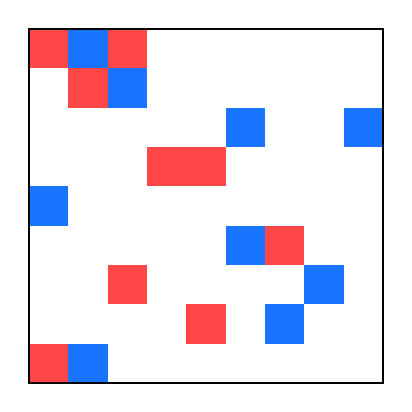
\begin{tikzpicture}[scale=0.5]
		\foreach \x / \y in {1/1,1/3,2/2,4/5,4/4,7/3,8/5,6/7,9/1} { \fill[red!90,opacity=.8] ({\y-1},{-\x+1}) rectangle +(1,-1);}
		\foreach \x / \y in {1/2,2/3,3/6,3/9,6/6,5/1,7/8,8/7,9/2} { \fill[blue!60!cyan,opacity=.9] ({\y-1},{-\x+1}) rectangle +(1,-1);}
%		\draw[semithick] (0,-9) grid (9,0);
		\draw[thick] (0,-9) rectangle (9,0);
	\end{tikzpicture}
\end{figure}


\end{frame}
\begin{frame}{Matrix partitioning}

Local view of the matrix for every processor:

	\begin{figure}[h]
	\centering
	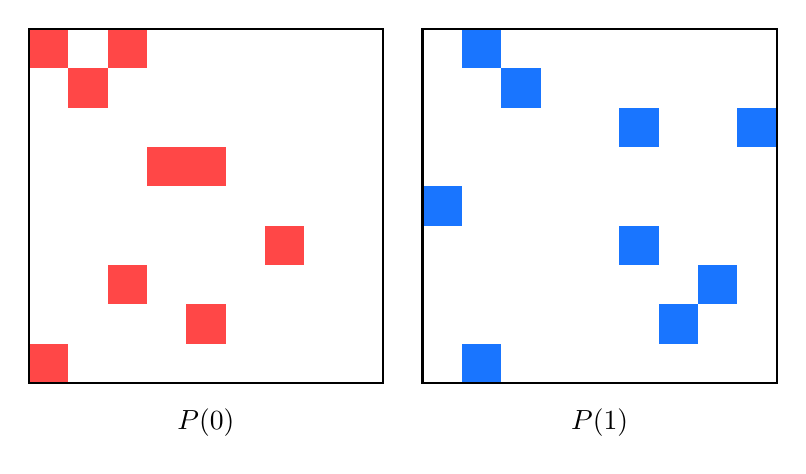
\begin{tikzpicture}[scale=0.5]
		\foreach \x / \y in {1/1,1/3,2/2,4/5,4/4,7/3,8/5,6/7,9/1} { \fill[red!90,opacity=.8] ({-10+\y-1},{-\x+1}) rectangle +(1,-1);}
		\foreach \x / \y in {1/2,2/3,3/6,3/9,6/6,5/1,7/8,8/7,9/2} { \fill[blue!60!cyan,opacity=.9] ({\y-1},{-\x+1}) rectangle +(1,-1);}
		\draw[thick] (-10,-9) rectangle (-1,0);
		\draw[thick] (0,-9) rectangle (9,0);
		\node at (-5.5,-10) {$P(0)$};
		\node at (4.5,-10) {$P(1)$};
	\end{tikzpicture}
\end{figure}


\end{frame}


\begin{frame}{Parallel matrix-vector multiplication algorithm}
		Parallel sparse matrix-vector multiplication is made (essentially) by 3 phases:

	\begin{enumerate}[I)]\itemsep=0.4cm
			\item \textbf{fan-out}%: each processor receives the required elements of $\vec{v}$ from the others (according to its distribution)
			\item \textbf{local multiplication}%: where the actual computation is performed
			\item \textbf{fan-in}%: where each processor sends his contributions to the other processors according to the distribution of $\vec{u}$
		\end{enumerate}
\end{frame}

\begin{frame}{Parallel matrix-vector multiplication algorithm}
	\begin{textblock}{170}(20,50)
		\only<1>{$A$ is partitioned along with $u$ and $v$}
		\only<2>{\textbf{Fan-out}:	each processor receives the required elements of $\vec{v}$ from the others (according to its distribution)}

		\only<3>{\textbf{Local multiplication}: where the actual computation is performed}

		\only<4>{\textbf{Fan-in}: where each processor sends his contributions to the other processors according to the distribution of $\vec{u}$}

\end{textblock}

	\begin{textblock}{100}(45,80)
	
	\begin{figure}[h]
	\centering
	\begin{tikzpicture}[scale=0.4]
		\foreach \x / \y in {1/1,1/3,2/2,4/5,4/4,7/3,8/5,6/7,9/1} { \fill[red!90,opacity=.8] ({\y-1},{-\x+1}) rectangle +(1,-1);}
		\foreach \x / \y in {1/2,2/3,3/6,3/9,6/6,5/1,7/8,8/7,9/2} { \fill[blue!60!cyan,opacity=.9] ({\y-1},{-\x+1}) rectangle +(1,-1);}

%		\draw[semithick] (0,-9) grid (9,0);
		\draw[thick] (0,-9) rectangle (9,0);

		\foreach \x in {2,4,5,7} { \fill[red!90,opacity=.8] ({\x-1},4) rectangle +(1,-1);}
		\foreach \x in {1,3,6,8,9} { \fill[blue!60!cyan,opacity=.9] ({\x-1},4) rectangle +(1,-1);}

\only<2>{
	\foreach \x in {1,3} { \draw[line width=2pt,blue!60!cyan,opacity=.9,->,>=latex] ({\x-0.5},2.8) -- ({\x-0.5},0.2);}
		\foreach \x in {2,7} { \draw[line width=2pt,red!90,opacity=.8,->,>=latex] ({\x-0.5},2.8) -- ({\x-0.5},0.2);}
	}
%	\draw[->,very thick,>=latex] ({7-0.5},1.8) -- ({7-0.5},{-7+0.2});
%		\draw[semithick] (0,3) grid (9,4);
		\draw[thick] (0,3) rectangle (9,4);

		\foreach \x in {2,4,6,7,9} { \fill[red!90,opacity=.8] (-4,{-\x+1}) rectangle +(1,-1);}
		\foreach \x in {1,3,5,8} { \fill[blue!60!cyan,opacity=.9] (-4,{-\x+1}) rectangle +(1,-1);}

\only<4>{		\foreach \x in {1,8} { \draw[line width=2pt,red!90,opacity=.8,->,>=latex] (-0.2,{-\x+0.5}) -- (-2.8,{-\x+0.5});}
		\foreach \x in {2,6,7,9} { \draw[line width=2pt,blue!60!cyan,opacity=.9,->,>=latex] (-0.2,{-\x+0.5}) -- (-2.8,{-\x+0.5});}
	}
%		\draw[semithick] (-4,-9) grid (-3,0);
		\draw[thick] (-4,-9) rectangle (-3,0);
		\node at (-3.5,-9.5) {$u$};
		\node at (9.5,3.5) {$v$};
		\node at (9.5,-9.5) {$A$};
	\end{tikzpicture}
\end{figure}
\end{textblock}
\end{frame}
\begin{frame}{Matrix partitioning}

	To optimize this process:

	\begin{itemize}
		\item I and III involve communication: it has to be \textbf{minimized}
		\item II is a computation step: we need \textbf{balance} in the size of the partitions
	\end{itemize}

	\textbf{Optimization problem}: partition the nonzeros such that the balance constraint is satisfied and the communication volume is minimized.

\end{frame}

\begin{frame}{Matrix partitioning}
	As a last example, a $6 \times 6$ ``checkerboard'' matrix:

	\begin{figure}[h]
	\centering
	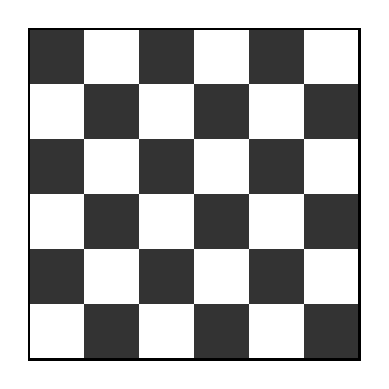
\begin{tikzpicture}[scale=0.7]
		\draw[thick] (0,0) rectangle (6,-6);
		\foreach \row in {0,1, ..., 5} {
			\foreach \column in {0, ..., 2} {
				\fill[opacity=.8] ({2*\column + mod(\row,2)}, -\row) rectangle +(1,-1);
			}
		};
%		\draw[semithick] (0,-6) grid (6,0);
	\end{tikzpicture}
\end{figure}

\end{frame}

\begin{frame}{Matrix partitioning}

	Two different partitionings result in extremely different communication volumes.

\begin{figure}[h]
	\centering
	\subfigure[Rows and columns are not split, therefore there is no need for communication.]{
		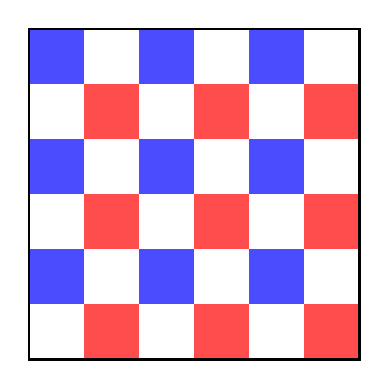
\begin{tikzpicture}[scale=0.7]
			\foreach \row in {0,2,4} {
				\foreach \column in {0, ..., 2} {
					\fill[opacity=.7,blue] ({2*\column + mod(\row,2)}, -\row) rectangle +(1,-1);
				}
			};
			\foreach \row in {1,3,5} {
				\foreach \column in {0, ..., 2} {
					\fill[opacity=.7,red] ({2*\column + mod(\row,2)}, -\row) rectangle +(1,-1);
				}
			};
%			\draw[semithick] (0,-6) grid (6,0);
			\draw[thick] (0,0) rectangle (6,-6);
		\end{tikzpicture} \label{fig:checkered_a}
	}\hspace{1cm}
	\subfigure[Every row and column is split and causes communication during fan-in and fan-out.]{
		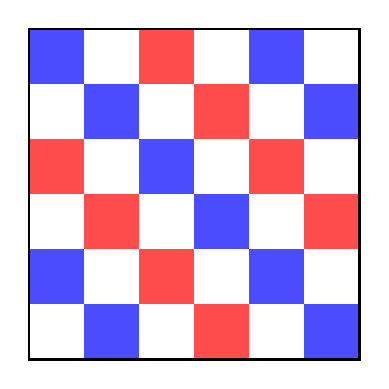
\begin{tikzpicture}[scale=0.7]
			\foreach \index in {0,1, ..., 5} {\fill[opacity=.7,blue] (\index, -\index) rectangle +(1,-1);};
			\foreach \index in {0,1, ..., 3} {\fill[opacity=.7,red] (2+\index, -\index) rectangle +(1,-1);};
			\foreach \index in {0,1, ..., 3} {\fill[opacity=.7,red] (\index, -2-\index) rectangle +(1,-1);};
			\foreach \index in {0,1} {\fill[opacity=.7,blue] (\index, -4-\index) rectangle +(1,-1);};
			\foreach \index in {0,1} {\fill[opacity=.7,blue] (4+\index, -\index) rectangle +(1,-1);};
%			\draw[semithick] (0,-6) grid (6,0);
			\draw[thick] (0,0) rectangle (6,-6);
		\end{tikzpicture} \label{fig:checkered_b}
	}
\end{figure}

\end{frame}

\subsection{Hypergraph partitioning}

\begin{frame}{Hypergraph partitioning}

Exact modeling of the matrix partitioning problem through \textbf{hypergraph partitioning}.

\begin{itemize}
	\item A partition of a hypergraph is simply the partition of the set of vertices $V$ into $V_0,\dots,V_{p-1}$.
	\item A hyperedge $e = \{v_1,\dots,v_k\}$ is \textbf{cut} if two of its vertices belong to different sets of the partition.
\end{itemize}

\end{frame}

\begin{frame}{Hypergraph partitioning}

	Hypergraph: a graph in which a \emph{hyperedge} can connect more than two \emph{vertices} (i.e. a subset of the vertex set $V$)

	\begin{figure}[h]
	\centering
\tikzstyle{vertex} = [fill,shape=circle,node distance=55pt]
\tikzstyle{edge} = [fill,opacity=.5,fill opacity=.5,line cap=round, line join=round, line width=50pt]
\tikzstyle{elabel} =  [fill,shape=circle,node distance=35pt]

\pgfdeclarelayer{background}
\pgfsetlayers{background,main}

\begin{tikzpicture}[scale=0.7,font=\small]
\node[vertex,label=above:\(v_1\)] (v1) {};
\node[vertex,right of=v1,label=above:\(v_2\)] (v2) {};
\node[vertex,below of=v1,label=above:\(v_4\)] (v4) {};
\node[vertex,right of=v4,label=above:\(v_5\)] (v5) {};
\node[vertex,left of=v4,label=above:\(v_3\)] (v3) {};
\node[vertex,below of=v4,label=above:\(v_7\)] (v7) {};
\node[vertex,left of=v7,label=above:\(v_6\)] (v6) {};

\begin{pgfonlayer}{background}
\draw[edge,color=blue] (v1) -- (v3) -- (v4) -- (v1);
\begin{scope}[transparency group,opacity=.5]
\draw[edge,opacity=1,color=green] (v4) -- (v7);
\end{scope}
\draw[edge,color=red] (v5) -- (v7);
\draw[edge,color=yellow] (v2) -- (v2);
\end{pgfonlayer}

\node[elabel,color=blue,label=right:{$e_1=\{v_1,v_3,v_4\}$}]  (e1) at (7,0) {};
\node[elabel,below of=e1,color=green,label=right:{$e_2=\{v_4,v_7 \}$}]  (e2) {};
\node[elabel,below of=e2,color=red,label=right:{$e_3=\left\{ v_5,v_7 \right\}$}]  (e3) {};
\node[elabel,below of=e3,color=yellow,label=right:{$e_4=\left\{ v_2 \right\}$}]  (e4) {};
\end{tikzpicture}
\end{figure}

\end{frame}


\begin{frame}{Hypergraph partitioning}

	There are several models to translate the matrix partitioning to hypergraph partitioning:

	\begin{itemize}
		\item 1-dimensional
		\begin{itemize}\itemsep=0.3cm
				\item\textbf{row-net}: each column of $A$ is a vertex in the hypergraph, each row a hyperedge. If $a_{ij} \neq 0$, then column $A_i$ is placed in the hyperedge $j$.
				\item \textbf{column-net}: identical to the previous one, with the roles of columns and rows exchanged
			\end{itemize}
			\vspace{0.5cm}
As hypergraph partitioning consists in assignment of the vertices, columns/rows are uncut. Advantage of eliminating completely one source of communication, but being 1-dimensional is often a too strong restriction.
\end{itemize}
\end{frame}

\begin{frame}{Hypergraph partitioning}
	\begin{itemize}
		\item 2-dimensional
			\begin{itemize}
					\vspace{0.2cm}
				\item \textbf{fine grain}: nonzeros of $A$ are vertices, rows and columns are hyperedges. The nonzero $a_{ij}$ is placed in the hyperedges $i$ and $j$

					\vspace{0.2cm}

				A lot of freedom in partitioning (each nonzero can be assigned individually), but the size of the hypergraph ($N$ vertices) is often too large.

					\vspace{0.2cm}
				\item \textbf{medium grain}: middle ground between 1-dimensional models and fine-grain

					\vspace{0.2cm}

					Good compromise between the size of the hypergraph and freedom during the partitioning.

			\end{itemize}
	\end{itemize}

\end{frame}

\subsection{The medium-grain method}

\begin{frame}{Medium grain}

	(Daniel M. Pelt and Rob Bisseling, 2013, to appear)

	\begin{figure}[h]
	\centering
	\begin{tikzpicture}[scale=0.2]%,font=\large]
\only<1>{		\foreach \x / \y in {1/1,1/3,2/2,4/5,4/4,3/11,4/9,6/7,1/10,2/7} { \fill[myblack] ({\y-1},{-\x+1}) rectangle +(1,-1);}
		\foreach \x / \y in {1/2,2/3,3/6,3/9,6/6,5/1,5/12,6/10,2/11,2/8} { \fill[myblack] ({\y-1},{-\x+1}) rectangle +(1,-1);}
		\draw[thick] (0,-6) rectangle (12,0);
		\node at (6,-7) {$A$};
	}
	\only<2->{	
		\foreach \x / \y in {1/1,1/3,2/2,4/5,4/4,3/11,4/9,6/7,1/10,2/7} { \fill[purple!90,opacity=.8] ({\y-1},{-\x+1}) rectangle +(1,-1);}
		\foreach \x / \y in {1/2,2/3,3/6,3/9,6/6,5/1,5/12,6/10,2/11,2/8} { \fill[yellow!60!cyan,opacity=.9] ({\y-1},{-\x+1}) rectangle +(1,-1);}
		\draw[thick] (0,-6) rectangle (12,0);
		\node at (6,-7) {$A$};
	}
		\visible<2->{
		\foreach \x / \y in {1/1,1/3,2/2,4/5,4/4,3/11,4/9,6/7,1/10,2/7}{ \fill[purple!90,opacity=.8] ({18+\y-1},{-6-\x+1}) rectangle +(1,-1);}
		\node at (24,-13) {$A_c$};
		\draw[thick] (18,{-6-6}) rectangle ({18+12},-6);

		\foreach \x / \y in  {1/2,2/3,3/6,3/9,6/6,5/1,5/12,6/10,2/11,2/8} { \fill[yellow!60!cyan,opacity=.9] ({18+\y-1},{6-\x+1}) rectangle +(1,-1);}
		\node at (24,-1) {$A_r$};
		\draw[thick] (18,{-6+6}) rectangle ({18+12},6);
		\draw[line width=1.3pt,>=latex,->] (13,-3) -- (17,-9);
		\draw[line width=1.3pt,>=latex,->] (13,-3) -- (17,3);
	}
\visible<3->{
	\foreach \x / \y in {1/1,1/3,2/2,4/5,4/4,3/11,4/9,6/7,1/10,2/7}{ \fill[purple!90,opacity=.8] ({36+\y-1},{-6-\x+1}) rectangle +(1,-1);}
	\foreach \x / \y in  {1/2,2/3,3/6,3/9,6/6,5/1,5/12,6/10,2/11,2/8} { \fill[yellow!60!cyan,opacity=.9] ({48+\x-1},{6-\y+1}) rectangle +(1,-1);}
	\draw[line width=1.3pt,>=latex,->] (31,-9) -- (35,-4);
		\draw[line width=1.3pt,>=latex,->] (31,3) -- (35,-2);


		\foreach \x in {1,2,3,9,10,11} { \fill[gray!10!black,opacity=.9] ({36+\x-1},{6-\x+1}) rectangle +(1,-1);}
		\foreach \x in {1,2,3,6} { \fill[gray!10!black,opacity=.9] ({48+\x-1},{-6-\x+1}) rectangle +(1,-1);}

		\draw[thick] (36,-12) rectangle (54,6);
		\draw[ultra thick] (48,-12) -- (48,6);
		\draw[ultra thick] (36,-6) -- (54,-6);

		\node at (45,-13) {$B$};
	}
		
	\end{tikzpicture}
\end{figure}

\vspace{-0.4cm}

\begin{itemize}

	\visible<2->{\item Initial split of $A$ into $A_c$ and $A_r$}
	\visible<3->{	\item Construction of the $(m+n)\times (m+n)$ matrix $B$ (with dummy diagonal elements)}
	\end{itemize}

\end{frame}


\begin{frame}{Medium grain}

\begin{figure}[h]
	\centering
%	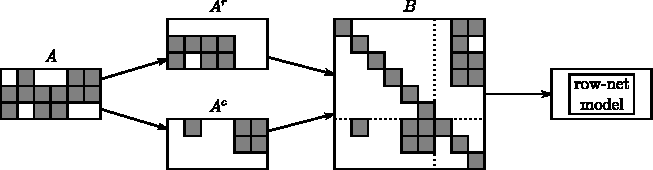
\includegraphics{img/mg-1}
	\begin{tikzpicture}[scale=0.2]

		\foreach \x / \y in {1/1,1/3,2/2,4/5,4/4,3/11,4/9,6/7,1/10,2/7}{ \fill[purple!90,opacity=.8] ({-34+\y-1},{-6-\x+1}) rectangle +(1,-1);}
		\foreach \x / \y in  {1/2,2/3,3/6,3/9,6/6,5/1,5/12,6/10,2/11,2/8} { \fill[yellow!60!cyan,opacity=.9] ({-22+\x-1},{6-\y+1}) rectangle +(1,-1);}


		\foreach \x in {1,2,3,9,10,11} { \fill[gray!10!black,opacity=.9] ({-34+\x-1},{6-\x+1}) rectangle +(1,-1);}
		\foreach \x in {1,2,3,6} { \fill[gray!10!black,opacity=.9] ({-22+\x-1},{-6-\x+1}) rectangle +(1,-1);}

	% \draw[very thin,help lines] (36,-12) grid (54,6);
		\draw[thick] (-34,-12) rectangle (-16,6);
		\draw[ultra thick] (-22,-12) -- (-22,6);
		\draw[ultra thick] (-34,-6) -- (-16,-6);

\visible<2->{		\draw[myarrow] (-15.5,-3) -- (-12.2,-3);
		\draw[thick] (-11.5,-6) rectangle (-4,0);
		\node at (-8,-2) {row-net};
		\node at (-8,-4) {model};

	}
	\visible<3->{
		\foreach \x / \y in {1/1,1/3,6/7,1/10,2/7}{ \fill[myred] ({0+\y-1},{-6-\x+1}) rectangle +(1,-1);}
		\foreach \x / \y in {2/2,4/5,4/4,4/9,3/11}{ \fill[myblue] ({0+\y-1},{-6-\x+1}) rectangle +(1,-1);}

		\foreach \x in {1,3,10} { \fill[myred] ({0+\x-1},{6-\x+1}) rectangle +(1,-1);}
		\foreach \x in {2,9,11} { \fill[myblue] ({0+\x-1},{6-\x+1}) rectangle +(1,-1);}

		\foreach \x / \y in  {1/2,2/3,3/6,3/9,6/6,5/1,5/12,6/10,2/11,2/8} { \fill[myred] ({12+\x-1},{6-\y+1}) rectangle +(1,-1);}
		\foreach \x / \y in  {2/3,6/6,6/10,2/11,2/8} { \fill[myblue] ({12+\x-1},{6-\y+1}) rectangle +(1,-1);}

		\foreach \x in {1,3} { \fill[myred] ({12+\x-1},{-6-\x+1}) rectangle +(1,-1);}
		\foreach \x in {2,6} { \fill[myblue] ({12+\x-1},{-6-\x+1}) rectangle +(1,-1);}

	%\draw[very thin,help lines] (0,-12) grid +(18,18);
		\draw[thick] (0,-12) rectangle +(18,18);
		\draw[ultra thick] (12,-12) -- +(0,18);
		\draw[ultra thick] (0,-6) -- +(18,0);

		\draw[myarrow] (-3.8,-3) -- (-0.5,-3);

	}
	\end{tikzpicture}
\end{figure}
	\visible<2->{
\begin{itemize}

\item Partitioning of $B$ with the row-net model (columns are kept together)
	\end{itemize}
}
\end{frame}

\begin{frame}{Medium grain}


	\begin{figure}[h]
	\centering
%	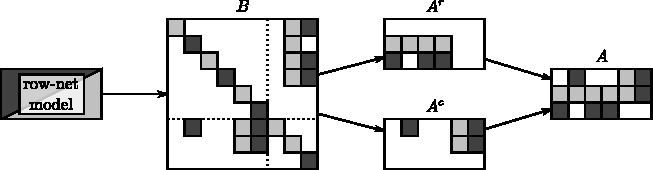
\includegraphics{img/mg-2}
	\begin{tikzpicture}[scale=0.2]
\visible<3->{
		\foreach \x / \y in {1/1,1/3,6/7,1/10,2/7}{ \fill[myred] ({42+\y-1},{-\x+1}) rectangle +(1,-1);}
		\foreach \x / \y in {2/2,4/5,4/4,4/9,3/11}{ \fill[myblue] ({42+\y-1},{-\x+1}) rectangle +(1,-1);}
		\foreach \x / \y in {1/2,3/6,3/9,5/1,5/12} { \fill[myred] ({42+\y-1},{-\x+1}) rectangle +(1,-1);}
		\foreach \x / \y in {2/3,6/6,6/10,2/11,2/8} { \fill[myblue] ({42+\y-1},{-\x+1}) rectangle +(1,-1);}
	%\draw[semithick] (42,-6) grid +(12,6);
		\draw[thick] (42,-6) rectangle +(12,6);

		\node at (48,-7) {$A$};
		\draw[myarrow] (37,-9) -- +(4,5);
		\draw[myarrow] (37,3) -- +(4,-5);
	}
	\visible<2->{
		\foreach \x / \y in {1/1,1/3,6/7,1/10,2/7}{ \fill[myred] ({24+\y-1},{-6-\x+1}) rectangle +(1,-1);}
		\foreach \x / \y in {2/2,4/5,4/4,4/9,3/11}{ \fill[myblue] ({24+\y-1},{-6-\x+1}) rectangle +(1,-1);}

		\node at (30,-13) {$A_c$};
	%\draw[semithick] (24,{-6-6}) grid +(12,6);
		\draw[thick] (24,{-6-6}) rectangle +(12,6);

		\foreach \x / \y in {1/2,3/6,3/9,5/1,5/12} { \fill[myred] ({24+\y-1},{6-\x+1}) rectangle +(1,-1);}
		\foreach \x / \y in {2/3,6/6,6/10,2/11,2/8} { \fill[myblue] ({24+\y-1},{6-\x+1}) rectangle +(1,-1);}
		\node at (30,-1) {$A_r$};
	%\draw[semithick] (24,{-6+6}) grid +(12,6);
			\draw[myarrow] (19,-3) -- +(4,6);
		\draw[myarrow] (19,-3) -- +(4,-6);
	\draw[thick] (24,{-6+6}) rectangle +(12,6);
	}

		\foreach \x / \y in {1/1,1/3,6/7,1/10,2/7}{ \fill[myred] ({0+\y-1},{-6-\x+1}) rectangle +(1,-1);}
		\foreach \x / \y in {2/2,4/5,4/4,4/9,3/11}{ \fill[myblue] ({0+\y-1},{-6-\x+1}) rectangle +(1,-1);}

		\foreach \x in {1,3,10} { \fill[myred] ({0+\x-1},{6-\x+1}) rectangle +(1,-1);}
		\foreach \x in {2,9,11} { \fill[myblue] ({0+\x-1},{6-\x+1}) rectangle +(1,-1);}

		\foreach \x / \y in  {1/2,2/3,3/6,3/9,6/6,5/1,5/12,6/10,2/11,2/8} { \fill[myred] ({12+\x-1},{6-\y+1}) rectangle +(1,-1);}
		\foreach \x / \y in  {2/3,6/6,6/10,2/11,2/8} { \fill[myblue] ({12+\x-1},{6-\y+1}) rectangle +(1,-1);}

		\foreach \x in {1,3} { \fill[myred] ({12+\x-1},{-6-\x+1}) rectangle +(1,-1);}
		\foreach \x in {2,6} { \fill[myblue] ({12+\x-1},{-6-\x+1}) rectangle +(1,-1);}

	%\draw[very thin,help lines] (0,-12) grid +(18,18);
		\draw[thick] (0,-12) rectangle +(18,18);
		\draw[ultra thick] (12,-12) -- +(0,18);
		\draw[ultra thick] (0,-6) -- +(18,0);

		\node at (9,-13) {$B$};
	\end{tikzpicture}

\end{figure}

	\visible<2->{
\begin{itemize}
\item Retrieval of $A_r$ and $A_c$ with the new partitioning
	\visible<3->{
\item Reassembling of $A$}
	\end{itemize}
}
\end{frame}

\begin{frame}{Medium grain}

	\begin{figure}
		\centering
		\begin{tikzpicture}[scale=0.3]
			\foreach \x / \y in {1/1,1/3,6/7,1/10,2/7}{ \fill[myred] ({42+\y-1},{-\x+1}) rectangle +(1,-1);}
		\foreach \x / \y in {2/2,4/5,4/4,4/9,3/11}{ \fill[myblue] ({42+\y-1},{-\x+1}) rectangle +(1,-1);}
		\foreach \x / \y in {1/2,3/6,3/9,5/1,5/12} { \fill[myred] ({42+\y-1},{-\x+1}) rectangle +(1,-1);}
		\foreach \x / \y in {2/3,6/6,6/10,2/11,2/8} { \fill[myblue] ({42+\y-1},{-\x+1}) rectangle +(1,-1);}
	%\draw[semithick] (42,-6) grid +(12,6);
		\draw[thick] (42,-6) rectangle +(12,6);

		\node at (48,-7) {$A$};
\end{tikzpicture}

\end{figure}
	\textbf{Clusters} of nonzeros are grouped together: 
	
	\begin{itemize}
		\item in $A_r$ we kept together elements of the same row;
		\item in $A_c$ elements of the same column.
	\end{itemize}

\end{frame}

\begin{frame}{Research directions}

%	Numerical experiments showed that the medium-grain method with \emph{Mondriaan} software partitionare gives good results.

	Two research directions:

\begin{itemize}
	\item Improving the initial partitioning of $A$
	\item Development of a fully iterative scheme: lowering the communication value by using information on the previous partitioning 
\end{itemize}

These directions can be combined: we can try to find efficient ways of splitting $A$ into $A_r$ and $A_c$, distinguishing between:

\begin{itemize}
	\item \emph{partition-oblivious} heuristics: no prior information is required
	\item \emph{partition-aware} heuristics: requirement of $A$ already partitioned
\end{itemize}
\end{frame}
